\documentclass{article}
\usepackage[utf8]{inputenc}

\usepackage{amsmath, amsthm, amsfonts, amssymb, stmaryrd}

\usepackage{tikz}

\theoremstyle{plain}
\newtheorem{theorem}{Theorem}
\newtheorem{lemma}[theorem]{Lemma}
\newtheorem{corollary}[theorem]{Corollary}
\newtheorem{proposition}[theorem]{Proposition}
\theoremstyle{definition}
\newtheorem{definition}[theorem]{Definition}
\newtheorem{example}[theorem]{Example}
\newtheorem{counter}[theorem]{Counterexample}
\theoremstyle{remark}
\newtheorem{remark}[theorem]{Remark}
\numberwithin{theorem}{section}

\newcommand{\ie}{\textit{i.e.}~}
\newcommand{\eg}{e.g.~}
\newcommand{\Fraisse}{Fra\"{i}ss\'{e}}
\newcommand{\set}{\mathsf{set}}
\newcommand{\GS}{S}
\newcommand{\As}{\mathcal{A}}
\newcommand{\Aso}{(\As, a_0)}
\newcommand{\Bs}{\mathcal{B}}
\newcommand{\Bso}{(\Bs, b_0)}
\newcommand{\Rs}{\mathcal{R}}
\newcommand{\Tr}{\mathsf{Tr}}
\newcommand{\preord}{\preceq}
\newcommand{\preford}{\sqsubseteq}
\newcommand{\op}{\mathsf{op}}
\newcommand{\Gd}{\mathbb{G}}
\newcommand{\Gk}{\mathbb{G}_{k}}
\newcommand{\Ek}{\mathbb{E}_{k}}
\newcommand{\Pk}{\mathbb{P}_{k}}
\newcommand{\Pd}{\mathbb{T}}
\newcommand{\IFF}{\Longleftrightarrow}
\newcommand{\rarr}{\rightarrow}
\newcommand{\id}{\mathsf{id}}
\newcommand{\sg}{\sigma}
\newcommand{\va}{\vec{a}}
\newcommand{\vb}{\vec{b}}
\newcommand{\vx}{\vec{x}}
\newcommand{\vy}{\vec{y}}
\newcommand{\vz}{\vec{z}}
\newcommand{\RA}{R^{\As}}
\newcommand{\RGA}{R^{\GG \As}}
\newcommand{\RB}{R^{\Bs}}
\newcommand{\RAB}{R^{\As \times \Bs}}
\newcommand{\ve}{\varepsilon}
\newcommand{\vempty}{\varnothing}
\newcommand{\vphi}{\varphi}
\newcommand{\gsim}{\preceq^{\gd}}
\newcommand{\gsimk}{\preceq^{\gd}_{k}}
\newcommand{\gbsim}{\sim^{\gd}}
\newcommand{\gbsimk}{\sim^{\gd}_{k}}
\newcommand{\vsa}{\vspace{.1in}}
\newcommand{\RS}{\mathcal{R}(\sg)}
\newcommand{\RSI}{\mathcal{R}(\sg +I)}
\newcommand{\RSIe}{\mathcal{R}(\sg +I^{=})}
\newcommand{\pref}{\sqsubseteq}
\newcommand{\upset}{{\uparrow}}
\newcommand{\downset}{{\downarrow}}
\newcommand{\covers}{\prec}
\newcommand{\IMP}{\; \Rightarrow \;}
\newcommand{\AND}{\; \wedge \;}
\newcommand{\Nat}{\mathbb{N}}
\newcommand{\Ss}{\mathscr{S}}
\newcommand{\incarrow}{\hookrightarrow}
\newcommand{\IGA}{I^{\Gd \As}}
\newcommand{\IGAB}{I^{\Gd (\As \times \Bs)}}
\newcommand{\RGAB}{R^{\Gd (\As \times \Bs)}}
\newcommand{\CS}{\mathsf{Struct}(\sg)}
\newcommand{\clique}{\mathsf{clique}}
\newcommand{\gd}{\mathfrak{g}}
\newcommand{\Gg}{\mathbb{G}^{\gd}}
\newcommand{\Gkg}{\mathbb{G}_{k}^{\gd}}
\newcommand{\GG}{\mathbb{G}}
\newcommand{\lb}{\llparenthesis}
\newcommand{\rb}{\rrparenthesis}
\newcommand{\epsA}{\ve_{\As}}
\newcommand{\dg}{\dagger}
\newcommand{\lt}{\langle}
\newcommand{\rt}{\rangle}
\newcommand{\gp}{\gamma^{+}}
\newcommand{\Guarded}{\mathsf{Guarded}}
\newcommand{\EMG}{\CS^{\GG}}
\newcommand{\EMGk}{\CS^{\Gk}}
\newcommand{\lrarr}{\leftrightarrow}

%Dan stuff
\newcommand{\hgraph}{\mathsf{HGraph}}
\newcommand{\hver}[1]{V_{#1}}
\newcommand{\hedg}[1]{E_{#1}}
\newcommand{\hyp}[1]{(\hver{#1},\hedg{#1})}
\newcommand{\HH}{\mathbb{H}}
\newcommand{\Hk}{\HH_{k}}
\newcommand{\until}{\mathbin{\mathbf{until}}}

\newcommand{\M}{\mathbb{M}}
\newcommand{\Mk}{\M_{k}}
\newcommand{\Mp}{\mathbb{M}^{\circlearrowright}}
\newcommand{\Mpk}{\Mp_{k}}

\newcommand{\N}{\mathbb{N}}
\newcommand{\Nk}{\N_{k}}

\newcommand{\A}{\mathbb{A}}
\newcommand{\Ak}{\A_{k}}

\title{Acyclicity and Neighbourhoods}
\author{Dan Marsden}
\date{August 2020}

\begin{document}

\maketitle

\section{Introduction}
This note is part of my efforts to understand Otto's work on acyclicity and amalgamation. As the body of work is large, and relatively complex, the aim is to find a simpler topic to build intuitions.
Specifically, we focus on some of the finite model theory proofs in~\cite{Otto2004} involving modal rather than guarded logics. We are particularly interested in expressive completeness proofs using finite model theoretic methods. The key ideas in~\cite{Otto2004} are (as I currently understand them):
\begin{itemize}
    \item Observation 13, which connects definability in a logic to finite approximations to logical equivalence.
    \item Definition 14, which introduces the key idea of upgrading notions of equivalence between models.
    \item The general observation that upgrading often requires some local good behaviour, and in general this can be approximated by bounded acyclicity.
\end{itemize}
For these reasons, we are interested in local restrictions of models, and unravelling constructions, particularly if they introduce some restricted acyclicity. This note observes that various constructions that seems to be of relevance are in fact comonads, although not directly motivated by model equivalence games. The aim then would be to develop a structural / categorical account of these proofs. This would involve understanding the interaction between these constructions and the bisimulation game comonads. The work in~\cite{Otto2004} goes as far as atom guarded logic in signatures of width two, and so this might provide a natural build up to the more general guarded situation.

For simplicity, we shall assume there is a single transition relation throughout, and we ignore unary propositions. This can be routinely generalized later.

\section{Comonads}

\subsection{Neighbourhoods}
Much of the arguments in~\cite{Otto2004} exploit models being locally well behaved. It is therefore useful to have a handle on neighbourhood restrictions of pointed structures. This comonad isn't particularly exciting on its own, but may provide a useful building block for local variants of other comonads.

\begin{proposition}[Neighbourhood Comonad]
For every~$k > 0$ there is a comonad on the category of pointed~$\sg$-structures with:
\begin{description}
\item[Action on Objects:] $\Nk\Aso$ is the induced substructure within distance at most~$k$ of~$a_0$ in the Gaifman graph.
\item[Counit:] $\epsilon_{\Aso}$ is the obvious embedding.
\item[Co-Kleisli Extension:] For~$f : \Nk\Aso \rightarrow \Bso$:
\begin{equation*}
    f^*(a) := f(a)
\end{equation*}
\end{description}
\end{proposition}
\begin{remark}
This is obviously an idempotent comonad, induced by the full subcategory of suitably local structures.
\end{remark}

\subsection{Partial Tree Unravelling}
Consider the pointed transition system~$\Aso$ depicted by:
\begin{equation}
    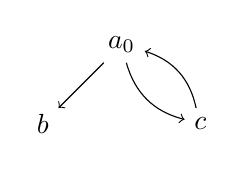
\begin{tikzpicture}
    \path 
    node (a) {$a_0$} +(-1,-1) 
    node (b) {$b$} +(1,-1) 
    node (c) {$c$};
    \path 
    (a) edge[->] (b) 
    (a) edge[->, bend right] (c)
    (c) edge[->, bend right] (a);
    \end{tikzpicture}
\end{equation}
The depth two unravelling given by the original comonad as~$\M_{2}\Aso$ is:
\begin{equation*}
    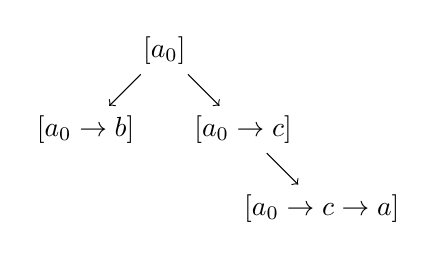
\begin{tikzpicture}
    \path 
    node (a) {$[a_0]$} +(-1,-1) 
    node (b) {$[a_0 \rightarrow b]$} ++(1,-1) 
    node (c) {$[a_0 \rightarrow c]$} ++(1,-1) 
    node (a') {$[a_0 \rightarrow c \rightarrow a]$};
    
    \path 
    (a) edge[->] (b) 
    (a) edge[->] (c)
    (c) edge[->] (a');
    \end{tikzpicture}
\end{equation*}
By construction, this is depth two bisimilar, but not bisimilar to the original structure. We write the lists used in the unravelling with rightward arrows rather than commas to smooth the potential transition to polymodal and bidirectional settings.

Our aim is a construction that is a tree up to a finite depth from the point, but is also fully bisimilar to the original transition system. To do this, we connect a copy of the original transition system at the bottom of the tree:
\begin{equation*}
    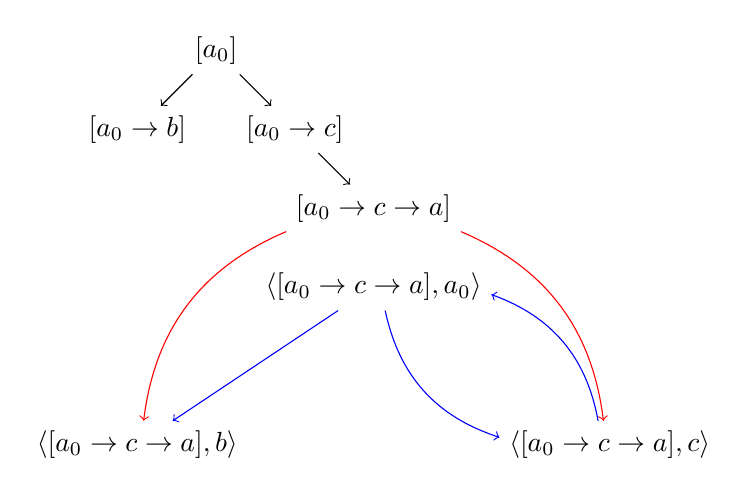
\begin{tikzpicture}
    \path 
    node (a) {$[a_0]$} +(-1,-1) 
    node (b) {$[a_0 \rightarrow b]$} ++(1,-1) 
    node (c) {$[a_0 \rightarrow c]$} ++(1,-1) 
    node (a') {$[a_0 \rightarrow c \rightarrow a]$} ++(0,-1)
    node (a*) {$\lt [a_0 \rightarrow c \rightarrow a], a_0 \rt$  } +(-3,-2) 
    node (b*) {$\lt [a_0 \rightarrow c \rightarrow a], b \rt$} +(3,-2) 
    node (c*) {$\lt [a_0 \rightarrow c \rightarrow a], c \rt $};
    
    \path 
    (a) edge[->] (b) 
    (a) edge[->] (c)
    (c) edge[->] (a')
    (a*) edge[blue, ->] (b*) 
    (a*) edge[blue, ->, bend right] (c*)
    (c*) edge[blue, ->, bend right] (a*)
    (a') edge[red, ->, bend right] (b*)
    (a') edge[red, ->, bend left] (c*);
    \end{tikzpicture}
\end{equation*}
Transitions in the copy appear in blue, and transitions from the unravelling to the copy appear in red.

Notice this gives a model that is a tree for~\emph{three} steps from the point of the structure. We have labelled our copy of the original structure with the path required to reach it, as in general there will be many such copies. This outline points towards the following construction:
\begin{proposition}[Partial Unravelling Comonad]
For each~$k \geq 0$, there is a comonad~$\Mpk$ on the category of pointed Kripke structures with:
\begin{description}
\item[Action on Objects:]~$\Mpk(\As,a_0)$ consists of paths~$[a_0 \rightarrow ... \rightarrow a_n]$ in~$\Aso$ starting at~$a_o$ and of length at most~$k + 1$, and pairs~$\lt p, a \rt$ where~$p = [a_0 \rightarrow \ldots \rightarrow a_k]$, there is an $\As$-edge originating at~$a_k$, and~$a \in \As$.
Relations are given as follows:
\begin{itemize}
    \item $R^{\Mpk\Aso}(p_1,p_2)$ if~$p_2$ extends~$p_1$ by one.
    \item $R^{\Mpk\Aso}(p, \langle p, a \rangle)$ if~$p = [a_0 \rightarrow \ldots \rightarrow a_k]$ and~$R^{\Aso}(a_k,a)$.
    \item $R^{\Mpk\Aso}(\langle p, a_1 \rangle, \langle p, a_2 \rangle)$ if~$R^{\Aso}(a_1,a_2)$.
\end{itemize}
\item[Counit:] On paths~$\epsilon_\As([a_0 \rightarrow \ldots \rightarrow a_n]) := a_n$, and on pairs~$\epsilon_\As (\langle p,a \rangle) := a$.
\item[Co-Kleisli Extension:] For~$f : \Mpk\Aso \rightarrow \Bso$:
\begin{itemize}
    \item On paths:
    \begin{equation*}
        f^* [a_0 \rightarrow \ldots \rightarrow a_n] := [f[a_0] \rightarrow \ldots \rightarrow f[a_0 \rightarrow \ldots \rightarrow a_n]]
    \end{equation*}
    \item On pairs:
    \begin{equation*}
        f^*(\lt p,a \rt) = \lt f^* p, f \langle p,a \rangle \rt
    \end{equation*}
\end{itemize}
\end{description}
\end{proposition}
\begin{remark}
Note that~$\Mp_{0}$ does one level of unravelling, not zero. It might be better to adjust the counting for this in a proper write up. For now, counting as above seems to make writing the definitions down slightly easier.
\end{remark}

\subsection{$k$-Acyclicity and Uniform Tree Unravelling}
The result of applying~$\Mpk$ is a limited form of acyclicity about the distinguished element. To achieve acyclicity more uniformly, we generalize the previous strategy, by ``unravelling everywhere''. For example, consider the (no longer pointed) transition system:
\begin{equation}
    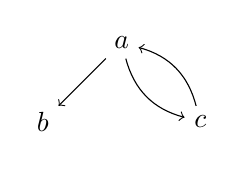
\begin{tikzpicture}
    \path 
    node (a) {$a$} +(-1,-1) 
    node (b) {$b$} +(1,-1) 
    node (c) {$c$};
    \path 
    (a) edge[->] (b) 
    (a) edge[->, bend right] (c)
    (c) edge[->, bend right] (a);
    \end{tikzpicture}
\end{equation}
Let us consider unravelling every state for two steps:
\begin{equation*}
    \begin{tikzpicture}
    \path 
    node (a) {$[a]$} +(-1,-1) 
    node (ab) {$[a \rightarrow b]$} ++(1,-1)
    node (ac) {$[a \rightarrow c]$} ++(1,-1)
    node (aca) {$[a \rightarrow c \rightarrow a]$} ++(0,-1)
    node (c') {$[c]$} ++(0,-1)
    node (c'a) {$[c \rightarrow a]$} +(-1,-1)
    node (c'ab) {$[c \rightarrow a \rightarrow b]$} +(1,-1)
    node (c'ac) {$[c \rightarrow a \rightarrow c]$} (b) ++(0,-2)
    node (b') {$[b]$};
    
    \path 
    (a) edge[->] (ab)
    (a) edge[->] (ac) 
    (ac) edge[->] (aca)
    (c') edge[->] (c'a)
    (c'a) edge[->] (c'ab)
    (c'a) edge[->] (c'ac);
    \end{tikzpicture}
\end{equation*}
So far, this is just a slight generalization of~$\M_{2}$ to unravel about every state, rather than just the distinguished element. So far, we haven't achieved much, but if we add some additional edges to allow final states to ``carry on at the start of the next tree'', we get:
\begin{equation*}
    \begin{tikzpicture}
    \path 
    node (a) {$[a]$} +(-1,-1) 
    node (ab) {$[a \rightarrow b]$} ++(1,-1)
    node (ac) {$[a \rightarrow c]$} ++(1,-1)
    node (aca) {$[a \rightarrow c \rightarrow a]$} ++(0,-1)
    node (c') {$[c]$} ++(0,-1)
    node (c'a) {$[c \rightarrow a]$} +(-1,-1)
    node (c'ab) {$[c \rightarrow a \rightarrow b]$} +(1,-1)
    node (c'ac) {$[c \rightarrow a \rightarrow c]$} (b) ++(0,-2)
    node (b') {$[b]$};
    
    \path 
    (a) edge[->] (ab)
    (a) edge[->] (ac) 
    (ac) edge[->] (aca)
    (c') edge[->] (c'a)
    (c'a) edge[->] (c'ab)
    (c'a) edge[->] (c'ac);
    
    \path[->,red]
    (aca) edge (b')
    (aca) edge (c')
    (c'ac.east) edge[out=0, in=90] (a.north);
    \end{tikzpicture}
\end{equation*}
Note that in each case, each list is fully bisimilar to its tail in the original structure. Also observe that the resulting structure has no cycles of length less than or equal to~\emph{three}.
\begin{remark}
The acyclicity seems obvious in the directed sense. For the undirected Gaifman graph, it also seems clear, but needs checking.
\end{remark}
This unravelling has lead us to the following construction:
\begin{proposition}[Acyclicity Comonad]
For each~$k \geq 0$ there is a comonad~$\Ak$ on Kripke structures, defined as follows:
\begin{description}
\item[Action on Objects:] $\Ak(\As)$ is the set of all non-empty paths of length at most~$k + 1$ in~$\As$. Relations are defined as follows:
\begin{itemize}
    \item $R^{\Ak(\As)}(p_1,p_2)$ if~$p_2$ extends~$p_1$ by one element.
    \item $R^{\Ak(\As)}([a_0 \rightarrow \ldots \rightarrow a_k], [a'_0])$ if~$R^{\As}(a_k, a'_0)$.
\end{itemize}
\item[Counit:] $\epsilon_{\As}$ is the tail function on non-empty sequences.
\item[Co-Kleisli Extension:] For~$f : \Ak(\As) \rightarrow \Bs$:
\begin{equation*}
    f^*([a_0 \rightarrow \ldots \rightarrow a_n] = [f([a_0]) \rightarrow \ldots \rightarrow f([a_0 \rightarrow \ldots \rightarrow a_n])]
\end{equation*}
\end{description}
\end{proposition}
\begin{remark}
The above construction removed the distinguished element to make the symmetry apparent. A pointed variant would also make sense, probably pruning some unreachable parts of the model.
\end{remark}

\section{Conclusion}
So far we have considered the most basic situation. Adding proposition variables should hopefully be routine. Also polymodal logics would require a move to transition labelled sequences, for example:
\begin{equation*}
    [a_0 \xrightarrow{\alpha} a_1 \xrightarrow{\beta} a_2]
\end{equation*}
Adapting to two-way bisimilarity would require the introduction of backward arrows:
\begin{equation*}
    [a_0 \xrightarrow{\alpha} a_1 \xleftarrow{\beta} a_2]
\end{equation*}
There may be some subtleties here to take care of, as we can now travel in both directions. As Otto points out, the two-way unravelling prunes forward-backward and backward-forward steps along the same relation, as these would introduce cycles in the Gaifman graph. 

We could also add global modalities by adding~$\xrightarrow{\forall}$ edges as have been considered previously for the game comonads, although again obviously details will need checking.

Otto considers more delicate constructions, using sufficiently acyclic groups. I suspect this is to get some sort of optimality in the constructions, although as this is preliminary work, there may be an omission somewhere.

\bibliography{main}
\bibliographystyle{alpha}

\end{document}
